% Task 8: brute force over short keys. c1 from Task8/crack.py; CHECKED with python3 and Task8/rc4.py:
%   c1 starts F3 CA 21 A4 C0; "Hello" = 48 65 6C 6C 6F
%   keystream(bytes([k]), 5) and the start of c1 XOR it:
%   00: de 18 89 41 a3 -> 2d d2 a8 e5 63     01: 06 08 0e 0e 18 -> f5 c2 2f aa d8
%   02: a4 01 06 a2 f3 -> 57 cb 27 06 33     03: 71 a2 11 d6 40 -> 82 68 30 72 80
%   ff: 6d 25 2f 24 70 -> 9e ef 0e 80 b0     (the right key is the result of the task: shown as ??)
%   256**5 = 1 099 511 627 776, 256**16 = 3.4e38
\documentclass[12pt,tikz,border=6pt]{standalone}
% Shared preamble of the task figures of Lecture 1.
% The colours and styles are copied from the preamble of ../main.tex (keep them in sync).
\usepackage{lmodern}
\usepackage[T1]{fontenc}
\renewcommand{\familydefault}{\sfdefault}
\usepackage{amsmath,amssymb}
\usepackage{xcolor}
\usepackage{fontawesome5}
\usetikzlibrary{arrows.meta, calc, positioning, fit, decorations.pathreplacing, decorations.pathmorphing, backgrounds}

% ---------- template ----------
\definecolor{DeepBlue}{HTML}{283593}
\definecolor{AccentOrange}{HTML}{EB5A14}
\definecolor{LightGray}{HTML}{F5F6FA}
% ---------- actors and categories (S1 to S6) ----------
\definecolor{sIndigo}{HTML}{5C6BC0}   % the sender
\definecolor{sPink}{HTML}{EC407A}     % the attacker
\definecolor{sViolet}{HTML}{7E57C2}   % plaintext
\definecolor{sAmber}{HTML}{FFB300}    % key and keystream
\definecolor{sTeal}{HTML}{26A69A}     % the receiver
\definecolor{sBrown}{HTML}{8D6E63}    % ciphertext
\definecolor{sPinkText}{HTML}{C2185B}
\definecolor{sAmberText}{HTML}{A06A00}
\definecolor{sTealText}{HTML}{00796B}
% ---------- actions and results ----------
\definecolor{aExec}{HTML}{43A047}
\definecolor{aRead}{HTML}{1E88E5}
\definecolor{aWrite}{HTML}{E53935}
% ---------- neutral ----------
\definecolor{nInk}{HTML}{37474F}
\definecolor{nLine}{HTML}{90A4AE}
\definecolor{nLight}{HTML}{CFD8DC}
\definecolor{nFill}{HTML}{ECEFF1}
\definecolor{nIdle}{HTML}{E0E0E0}

% ---------- TikZ styles (as in main.tex; byte cells a little larger for the web) ----------
\tikzset{
  hw/.style={draw=nLine, thick, fill=nFill, text=nInk, rounded corners=3pt, align=center, inner sep=4pt},
  hwmain/.style={draw=nInk, thick, fill=nInk, text=white, rounded corners=3pt, align=center, inner sep=4pt},
  cell/.style={draw=nLine, thick, fill=white, text=nInk, font=\ttfamily\small},
  cellfree/.style={cell, dashed, draw=nLight},
  container/.style={draw=nLine, thick, dashed, rounded corners=5pt},
  actor/.style={fill=#1, draw=#1, text=white, rounded corners=3pt, align=center, font=\small\bfseries, inner sep=5pt},
  actorlight/.style={fill=#1!15, draw=#1, thick, text=nInk, rounded corners=3pt, align=center, inner sep=5pt},
  data/.style={-{Stealth}, very thick, nInk},
  flow/.style={-{Stealth}, very thick, DeepBlue},
  annot/.style={draw=AccentOrange, line width=1.6pt, rounded corners=3pt},
  byte/.style={draw=nLine, thick, fill=white, text=nInk, font=\ttfamily\small,
    minimum width=0.8cm, minimum height=0.62cm, inner sep=1pt, rounded corners=1.5pt},
  ptb/.style={byte, fill=sViolet!15, draw=sViolet},
  ksb/.style={byte, fill=sAmber!25, draw=sAmber},
  ctb/.style={byte, fill=sBrown!15, draw=sBrown},
  unk/.style={byte, fill=white, dashed, text=sViolet},
  rowlabel/.style={font=\small\bfseries, text=nInk, anchor=east},
  note/.style={font=\small, text=nInk},
  bigxor/.style={circle, draw=nInk, very thick, fill=white, inner sep=0pt, minimum size=0.8cm, font=\Large},
  radio/.style={-{Stealth}, very thick, nInk, decorate,
    decoration={snake, amplitude=1.2pt, segment length=7pt, post length=4pt}},
  % a white card behind the whole figure, so that it stays readable in a dark theme
  card/.style={show background rectangle, background rectangle/.style={fill=white, draw=none}, inner frame sep=8pt},
}
% a row of bytes: \byterow{x of the first cell}{y}{style}{list of values}{step between cells}
\newcommand{\byterow}[5]{%
  \expandafter\def\expandafter\brlist\expandafter{#4}%
  \foreach \v [count=\k from 0] in \brlist {
    \node[#3] at ({#1+#5*\k},#2) {\v};
  }}
% the generator / cipher box: dark, with cogs. \cogbox{name}{position}{label}{width}
\newcommand{\cogbox}[4]{%
  \node[hwmain, minimum width=#4, minimum height=1.3cm] (#1) at (#2) {};
  \node[text=white, font=\Large] at ([yshift=0.22cm]#1.center) {\faCogs};
  \node[text=white, font=\small\bfseries] at ([yshift=-0.32cm]#1.center) {#3};}
\newcommand{\ok}{\textcolor{aExec}{\faCheck}}
\newcommand{\nok}{\textcolor{aWrite}{\faTimes}}
\newcommand{\badge}[1]{\tikz[baseline=(b.base)]\node[circle,fill=AccentOrange,text=white,
  inner sep=1.5pt,font=\bfseries\footnotesize] (b) {#1};}

\begin{document}
\pagecolor{white}
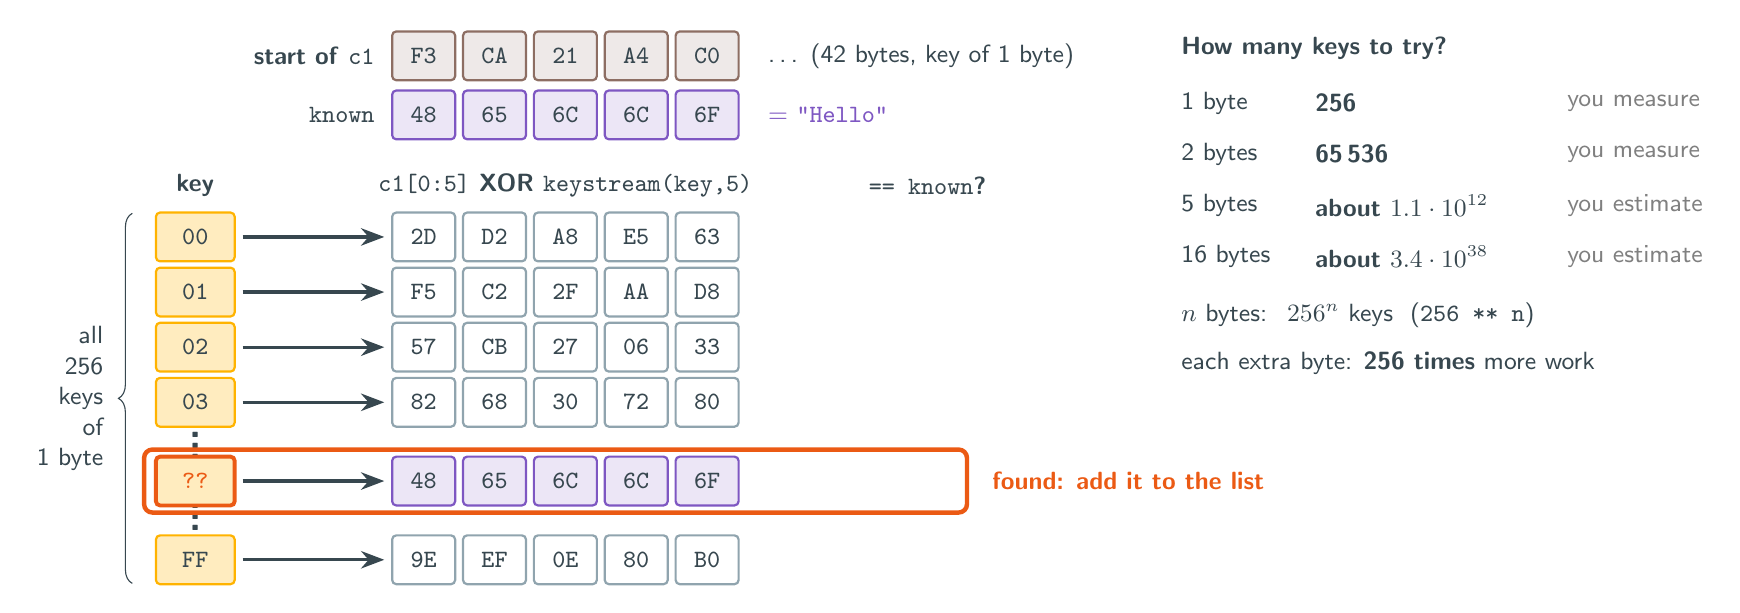
\begin{tikzpicture}[>=Stealth]
  \def\dx{0.9}
  \tikzset{kb/.style={byte, fill=sAmber!25, draw=sAmber, minimum width=1.0cm, font=\ttfamily\small\bfseries},
           rb/.style={byte, minimum width=0.8cm}}
  % the start of the ciphertext and the known start
  \node[rowlabel] at (3.0,3.0) {start of \texttt{c1}};
  \byterow{3.5}{3.0}{ctb}{F3,CA,21,A4,C0}{\dx}
  \node[note, anchor=west] at (7.75,3.0) {\ldots\ (42 bytes, key of 1 byte)};
  \node[rowlabel] at (3.0,2.25) {\texttt{known}};
  \byterow{3.5}{2.25}{ptb}{48,65,6C,6C,6F}{\dx}
  \node[note, anchor=west, text=sViolet] at (7.75,2.25) {= \texttt{"Hello"}};

  % the loop over all keys
  \node[font=\small\bfseries, text=nInk] at (0.6,1.35) {key};
  \node[font=\small\bfseries, text=nInk] at (5.3,1.35) {\texttt{c1[0:5]} XOR \texttt{keystream(key,5)}};
  \node[font=\small\bfseries, text=nInk] at (9.9,1.35) {\texttt{== known}?};
  \foreach \y/\k/\v/\r in {0.7/00/{2D,D2,A8,E5,63}/0, 0.0/01/{F5,C2,2F,AA,D8}/0, -0.7/02/{57,CB,27,06,33}/0,
                           -1.4/03/{82,68,30,72,80}/0, -3.4/FF/{9E,EF,0E,80,B0}/0} {
    \node[kb] at (0.6,\y) {\k};
    \draw[data] (1.2,\y) -- (3.0,\y);
    \byterow{3.5}{\y}{rb}{\v}{\dx}
    \node[font=\large] at (9.9,\y) {\nok};
  }
  \foreach \y in {-1.95,-2.85} \node[font=\Large\bfseries, text=nInk] at (0.6,\y+0.1) {$\vdots$};
  \node[kb, draw=AccentOrange, line width=1.4pt, text=AccentOrange] at (0.6,-2.4) {??};
  \draw[data] (1.2,-2.4) -- (3.0,-2.4);
  \byterow{3.5}{-2.4}{ptb}{48,65,6C,6C,6F}{\dx}
  \node[font=\large] at (9.9,-2.4) {\ok};
  \draw[annot] (-0.05,-2.8) rectangle (10.4,-2.0);
  \node[font=\small\bfseries, text=AccentOrange, anchor=west] at (10.6,-2.4) {found: add it to the list};
  \draw[decorate, decoration={brace, mirror, amplitude=5pt}, nInk] (-0.2,1.0) -- (-0.2,-3.7)
    node[midway, left=7pt, note, align=right] {all\\256\\keys\\of\\1 byte};

  % how many keys
  \begin{scope}[shift={(13.3,3.1)}]
    \node[font=\small\bfseries, text=nInk, anchor=west] at (-0.3,0) {How many keys to try?};
    \foreach \y/\n/\c/\t in {-0.7/1 byte/256/you measure, -1.35/2 bytes/65\,536/you measure,
                             -2.0/5 bytes/about $1.1 \cdot 10^{12}$/you estimate, -2.65/16 bytes/about $3.4 \cdot 10^{38}$/you estimate} {
      \node[font=\small, text=nInk, anchor=west] at (-0.3,\y) {\n};
      \node[font=\small\bfseries, text=nInk, anchor=west] at (1.4,\y) {\c};
      \node[font=\small, text=gray, anchor=west] at (4.6,\y) {\t};
    }
    \node[font=\small, text=nInk, anchor=west] at (-0.3,-3.4) {$n$ bytes: \ $256^n$ keys \ (\texttt{256 ** n})};
    \node[font=\small, text=nInk, anchor=west] at (-0.3,-4.0) {each extra byte: \textbf{256 times} more work};
  \end{scope}
\end{tikzpicture}
\end{document}
